\documentclass{article}

% Configurações Genéricas ------------------------------------------------------
\usepackage[utf8]{inputenc}
\usepackage[T1]{fontenc}
\usepackage[brazil]{babel}
\usepackage{sbc-template}
\usepackage{graphicx}

% Informações Pessoais ---------------------------------------------------------
\title{Tarefa 05 sobre Desenvolvimento com Android}
\author{Wanderson Henrique Camargo Rosa\inst{1}}
\address{Programação para Dispositivos Móveis 2011/1\\Centro de Ciências Exatas
e Tecnológicas\\Universidade do Vale do Rio dos Sinos ---
UNISINOS\email{wandersonwhcr@gmail.com}}

% Documento --------------------------------------------------------------------
\begin{document}

\maketitle{}

% Introdução -------------------------------------------------------------------
\section{Introdução}
\label{sec:introducao}

O presente documento é resultado da quinta tarefa sobre desenvolvimento em
dispositivos móveis. Há a necessidade de criação de um aplicativo sobre a
plataforma Android que utilize um objeto do tipo \texttt{MapView} ou
\texttt{WebView} e que seja simples e funcional.

A Seção \ref{sec:idealizacao} exibe uma primeira análise sobre o componente
utilizado nesta tarefa. Já a Seção \ref{sec:implementacao} mostra como os
objetos foram criados e relacionados para formar o aplicativo. A Seção
\ref{sec:icones} informa sobre como podemos utilizar os ícones padrão
disponíveis no Sistema Operacional Android. Ao final, as Seções
\ref{sec:execucao} e \ref{sec:finais} demonstram como o aplicativo se comportou
em tempo de execução e quais serão os próximos passos do desenvolvimento do
Trabalho de Grau A desta disciplina.

% Idealização ------------------------------------------------------------------
\section{Idealização}
\label{sec:idealizacao}

Pensando em utilizar um destes componentes no Projeto do Grau A, posso incluir
um objeto da classe \texttt{WebView} para exibir páginas contendo informações
sobre o aplicativo e auxílios de como utilizá-lo. Acessando arquivos locais,
será possivel navegar na documentação disponível e verificar como podem ser
executadas as tarefas sobre o programa, sem uma conexão de dados externa.

\subsection{Análise Primária}

Após trabalhar com alguns \emph{tutoriais} disponíveis, percebi que a utilização
do componente de visualização de páginas HTML \texttt{WebView} não aparentava
ser complicado. Para aplicar as idéias iniciais, precisamos criar uma atividade
que receba este componente e que irá capturar os comandos fornecidos pelo
usuário.

% Implementação ----------------------------------------------------------------
\section{Implementação}
\label{sec:implementacao}

Foram adicionadas duas atividades após a criação de um novo projeto para testes.
A \texttt{MainActivity} recebeu um menu de contexto para acessar as informações
de ajuda, conforme Figura \ref{fig:main}. Estas informações são requisitadas
através de uma intenção ao sistema, solicitando a atividade
\texttt{AboutActivity}, que contém o componente de visualização de páginas HTML.

\begin{figure}
    \centering{}
    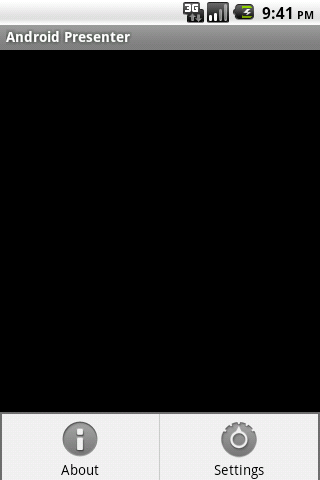
\includegraphics[scale=0.4]{figura01.png}
    \caption{Atividade Principal com Menu de Contexto}
    \label{fig:main}
\end{figure}

Nesta atividade foi inicializado um objeto do tipo \texttt{WebView} em tempo de
criação. A linguagem Javascript foi desabilitada porque não haverá necessidade
de interpretação de comandos pela simplicidade das páginas.

\subsection{Sobrescrita ao Cliente de Acesso}

Um objeto do tipo \texttt{WebView} cria uma nova intenção ao sistema para abrir
o navegador padrão sempre que um \emph{hyperlink} é acessado. Para que o próprio
objeto de visualização abra esta nova página, foi adicionada uma classe aninhada
privada \texttt{AboutWebViewClient}, estendida da classe
\texttt{WebViewClient}, onde há uma sobrescrita do método que carrega novas
páginas.

Um novo objeto desta classe foi incluído no componente de visualização para
trabalhar com \emph{hyperlinks} internamente.

\subsection{Páginas Locais}

Por motivos de simplicidade, não é necessário que as páginas sobre o aplicativo
sejam acessadas através de uma conexão de dados. Estas podem ser armazenadas
dentro do aplicativo e acessíveis utilizando um endereço específico. Podemos
verificar sua utilização na Figura \ref{fig:about}.

\begin{figure}
    \centering{}
    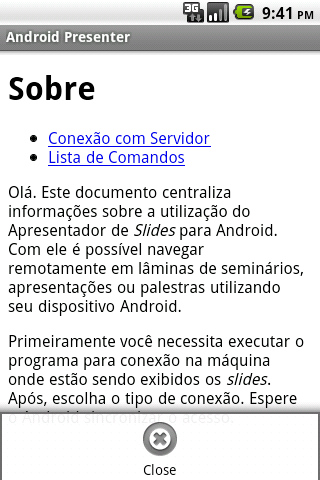
\includegraphics[scale=0.4]{figura02.png}
    \caption{Componente de Visualização de Páginas com Menu de Contexto}
    \label{fig:about}
\end{figure}

Existe um diretório chamado \texttt{assets} que armazena arquivos completos que
não são utilizados em tempo de compilação, portanto não geram identificadores na
classe de ponteiros aos recursos estáticos \texttt{R}.

Podemos armazenar os arquivos no formato HTML e acessá-los utilizando o endereço
\texttt{file:///android\_asset}. Por exemplo, a página inicial,  do componente é
armazenada no diretório \texttt{assets/about.html} e acessível pelo objeto de
visualização através do endereço \texttt{file:///android\_asset/about.html}.

Foram desenvolvidas duas páginas, \texttt{about.html} e \texttt{server.html},
com \emph{hyperlinks} circulares para confirmar a navegação interna ao
componente. Como não há necessidade de acesso a páginas externas, não foi
necessária adição de permissões exclusivas ao aplicativo.

\subsection{Navegação}

Conforme a navegação entre páginas é executada, há a possibilidade de retorno no
histórico utilizando o próprio componente de visualização e a captura de teclas
na atividade.

O método responsável pelo tratamento de teclas pressionadas no dispositivo foi
sobrescrito na atividade. Quando a tecla \emph{voltar} é acionada, a sua
operação padrão é anulada caso existam páginas no visualização anteriormente
visitadas.

Porém, quando o usuário visita muitas páginas, é inviável que ele volte todo o
histórico somente para finalizar a atividade atual. Evitando este problema, a
atividade \texttt{AboutActivity} recebeu um menu de contexto contendo um item
que possibilita a sua finalização, visível na Figura \ref{fig:about}.

% Ícones Internos ao Android ---------------------------------------------------
\section{Ícones Internos ao Android}
\label{sec:icones}

Buscando padronização dos aplicativos, houve a necessidade de utilização dos
próprios ícones dos aplicativos Android no projeto. Após pesquisa sobre o
assunto e navegação no código-fonte do Sistema Operacional, encontrei ícones
diversos no formato PNG que são utilizados pelas \emph{interfaces}.

Como não consegui utilizar o GIT para efetuar uma cópia do diretório, busquei
\emph{tutoriais} sobre o assunto e \emph{sites} para visualização dos ícones.

\subsection{Utilização}

Para referenciar os ícones internos, basta utilizar um ponteiro com seu nome
prefixado com o endereço \texttt{@android:drawable/}. Por exemplo, para utilizar
o ícone que representa uma informação no sistema chamado
\texttt{ic\_menu\_info\_details}, basta utilizar um ícone com a referência
\texttt{@android:drawable/ic\_menu\_info\_details}.

% Execução ---------------------------------------------------------------------
\section{Execução}
\label{sec:execucao}

Esta versão de testes foi testada no emulador disponível pelo ambiente de
desenvolvimento e no \emph{smartphone} Samsung Galaxy 5 com Android 2.2 Froyo,
conforme Figura \ref{fig:smart}. O aplicativo foi gerado da mesma forma
utilizada nos relatórios anteriores. Não houve erros devido a sua simplicidade.

\begin{figure}
    \centering{}
    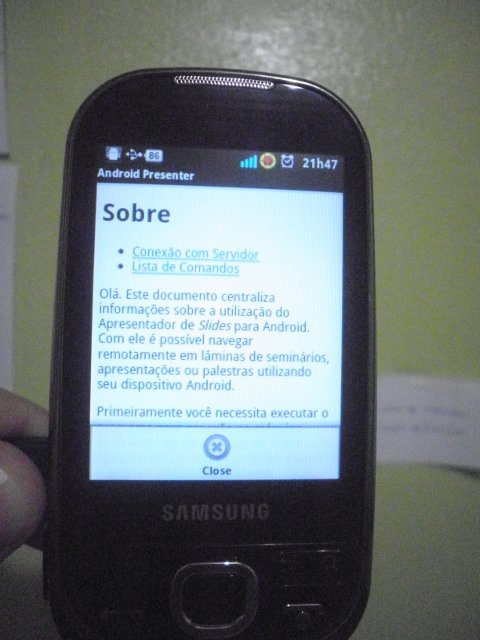
\includegraphics[scale=0.3]{figura03.jpg}
    \caption{Aplicativo Executando sobre um \emph{Smartphone}}
    \label{fig:smart}
\end{figure}

% Anotações Finais -------------------------------------------------------------
\section{Anotações Finais}
\label{sec:finais}

Com o passar do tempo, o ambiente de desenvolvimento em Android começa a se
tornar mais claro e de fácil utilização, já que a estrutura necessita ser um
pouco rígida. Como estamos trabalhando há 3 semanas nesta tecnologia, a criação
deste aplicativo foi muito rápida em comparação com os anteriores.

A busca de informações sobre o componente \texttt{WebView} durou cerca de 1h. A
criação da estrutura de classes que representam atividades levou 20min para ser
completada. A pesquisa sobre diretório e leitura de arquivos estáticos foi
finalizada em 30min, juntamente com a criação das duas páginas com informações
sobre o aplicativo. Informações sobre a utilização de ícones padrão do Android
foram encontradas em 1h30min. A documentação final levou 1h30min para ser
escrita. Portanto, foram utilizadas cerca de 4h50min para finalização desta
tarefa, distribuídas entre os dias 4 e 5 de abril de 2011.

\subsection{Continuidade do Projeto}

Os códigos desenvolvidos nesta tarefa serão melhor estudados e incluídos no
Trabalho de Grau A desta disciplina. Eles servirão como arquivos de ajuda para
usuários que buscam mais informações sobre a utilização do aplicativo.

\end{document}